\chapter{Photon Mapping}
Although radiosity is very efficient to render indirect lighting, it only considers diffuse surfaces. We want an algorithm capable of handling any type of BRDF. Besides, radiosity methods suffer from mesh artifacts (the sharp edges).

Photon Mapping, was invented by Henrik Wann Jensen\cite{a:GlobalIlluminationusingPhotonMaps} to speedup Monte Carlo ray tracing. The idea is to change the representation of the illumination. Instead of tightly coupling lighting information with the geometry, the information is stored in a separate independent data structure, the \textit{photon map}. The photon map is constructed from photons emitted from the light sources and traced through the model. It contains information about all photon hits, and this information can be used to efficiently render the model. The decoupling of the photon map from the geometry is a significant advantage that not only simplifies the representation but also makes it possible to use the structure to represent lighting in very complex models. The combination of photon mapping and a Monte Carlo ray-tracing-based rendering algorithm results in an algorithm that is as general as pure Monte Carlo ray tracing but significantly more efficient.

Unlike path tracing, photon mapping is a "biased" rendering algorithm, which means that the average expected values of the method may not be the correct solution to the rendering equation. However, since it is a consistent method, any desired accuracy can be achieved by increasing the number of photons.




\section{Regular Photon Mapping}
Photon Mapping comes from the earlier \textit{photon density estimation} technique which proposed by Arvo in his backward ray tracing method\cite[-3mm]{a:Backwardraytracing}. Arvo's approach first distributes packets of light energy across the scene using photon tracing. It then computes the local density using the histogram method, by counting the number of photons in discrete bins on surfaces, to estimate the lighting intensity. 

Since then, photon density estimation has attracted great interests from the research community due to its generality. The most successful photon density estimation algorithms is photon mapping\cite{a:GlobalIlluminationusingPhotonMaps}. Photon mapping uses k-NN (k-nearest neighbour) density estimation and was the first to use photon density estimation for view-independent rendering. Photon mapping also popularized the concept of the two pass approach to photon density estimation.



\subsection{Photon Tracing}
The purpose of the photon tracing pass is to compute indirect illumination on diffuse. This is done by emitting photons from the light sources, tracing them through the scene, and storing them at diffuse.


\subsubsection{Photon Emission}
What is a photon? The photons emitted from a light source and have a distribution corresponding to the distribution of emissive power of the light source. A photon carries flux (power), not radiance! It is a fraction of the light source power and several wavelengths combined into one entity. Given $\Phi$ watt lightbulb, emit $N$ photons, each photon has the power $\frac{\Phi}{N}$ watt. Photon power depends on the number of emitted photons.

In general, the light source can have any shape and emission characteristics -- the intensity of the emitted light varies with both origin and direction. 

\begin{figure}\label{f:photon-emission}
	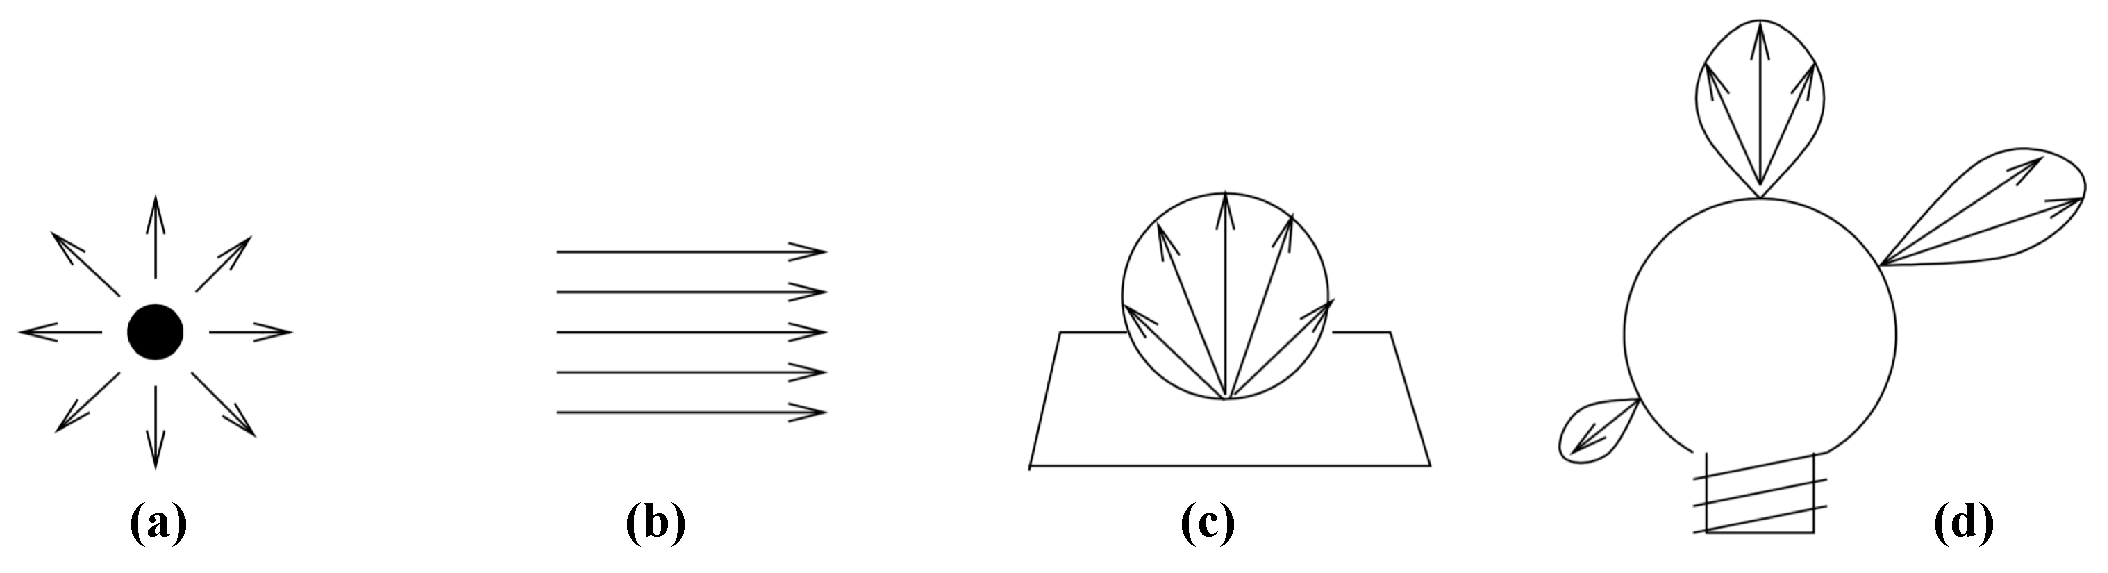
\includegraphics[width=1.0\textwidth]{graphics/pm/pm-3}
	\caption{Emission from light sources: (a) point light, (b) directional light, (c) square light, (d) general light.}
\end{figure}

For example, photons from a diffuse point light source are emitted in uniformly distributed random directions from the point, see algorithm \ref{lst:diffuse-point-light}. Photons from a directional light are all emitted in the same direction, but from origins outside the scene. Photons from a diffuse square light source are emitted from random positions on the square, with directions limited to a hemisphere. The emission directions are chosen from a cosine distribution: there is zero probability of a photon being emitted in the direction parallel to the plane of the square, and highest probability of emission is in the direction perpendicular to the square. Figure \ref{f:photon-emission} shows the emission from these different types of light sources.

\begin{algorithm}\label{lst:diffuse-point-light}
\begin{lstlisting}[language=C++, mathescape]
emit_photons_from_diffuse_point_light() {
	$n_e = 0$ //number of emitted photons 
 	while (not enough photons) {
		do { //use simple rejection sampling to find diffuse photon direction 
 			x = random number between -1 and 1
			y = random number between -1 and 1
			z = random number between -1 and 1
		} while ( $x^{2} + y^{2} + z^{2} > 1$ )
		$\vec{d}$ = < x , y , z >
		$\vec{p}$ = light source position
		trace photon from $\vec{p}$ in direction $\vec{d}$ 
 		$n_e =n_e +1$
	}
	scale power of stored photons with $1/n_e$ 
}
\end{lstlisting}
\caption{Pseudocode for emission of photons from a diffuse point light}
\end{algorithm}



\subsubsection{Photon Scattering}
Once a photon has been emitted, it is traced through the scene using photon tracing. Photon tracing works in exactly the same way as ray tracing except for the fact that photons propagate flux whereas rays gather radiance. When a photon hits an object, it can either be reflected, transmitted, or absorbed. That is decided probabilistically based on the material parameters of the surface.

\begin{figure}
\sidecaption
	\includegraphics[width=.65\textwidth]{graphics/pm/pm-4}
	\caption{Photon paths in a scene (a "Cornell box" with a chrome sphere on left and a glass sphere on right): (a) two diffuse reflections followed by absorption, (b) a specular reflection followed by two diffuse reflections, (c) two specular transmissions followed by absorption.}
\end{figure}

If a photon hits a mirror surface a new photon is reflected in the mirror direction. Given a normal, $\vec{n}$, and an incoming direction, $\vec{\omega}^{'}$, the reflected direction, $\vec{\omega}$, is found as:

\begin{equation*}
	\vec{\omega}=2(\vec{n}\cdot\vec{\omega}^{'})\vec{n}-\vec{\omega}^{'}
\end{equation*}

where the incoming direction is assumed to point away from the intersection point. This equation is the same that is used in ray tracing to trace specularly reflected rays. The power of the reflected photon should be scaled by the reflectivity of the mirror (unless Russian roulette sampling is used).

When a photon hits a diffuse surface it is stored in the photon map. The direction of the diffusely reflected photon (from a Lambertian surface) is found by picking a random direction in the hemisphere above the intersection point with a probability proportional to the cosine of the angle with the normal. The power of the reflected photon is found by scaling the power of the incoming photon with the diffuse reflectance (unless Russian roulette sampling is used).

Given an arbitrary BRDF the new photon direction should be computed by importance sampling the BRDF. For several reflection models the importance-sampling function can be found analytically.


\subsubsection{Photon Storing}
As already mentioned photons are stored only when they hit diffuse surface. The reason is that storing photons on specular surfaces does not give any useful information: the probability of having a matching incoming photon from the specular direction is small (and zero for perfect specular materials); so, if we want to render accurate specular reflections, the best way is to trace a ray in the mirror direction using standard ray tracing, see section \ref{sec:photon-mapping-rendering}. For all other photon-surface intersections, data is stored in a global data structure, the \textit{photon map}.

It is important to realize that photons represent incoming illumination (flux) at a surface. This is a valuable optimization that enables us to use a photon to approximate the \textit{reflected} illumination at several points on a surface.

\begin{figure}\label{f:photon-storing}
\begin{center}
	\begin{subfigure}[b]{0.492\textwidth}
		\includegraphics[width=1.0\textwidth]{graphics/pm/pm-2-1}
	\end{subfigure}
	\begin{subfigure}[b]{0.492\textwidth}
		\includegraphics[width=1.0\textwidth]{graphics/pm/pm-2-2}
	\end{subfigure}
\end{center}
\caption{"Cornell box" with glass and chrome spheres: (a) ray traced image (direct illumination and specular reflection and transmission), (b) the photons in the corresponding photon map.}
\end{figure}

Figure \ref{f:photon-storing} shows the stored photons (estimated flux density) in the box scene. Notice how the photons estimate the incoming illumination and how the density is higher in regions with strong incoming illumination, such as for the caustic below the glass sphere.



\subsection{The Photon Map Data Structure}
The photon map is a representation of all the stored photons in the model. A fundamental aspect of the photon map is that it is decoupled from the geometry. This means that we do not associate photons with certain geometry, but instead keep them in a separate structure.


\subsubsection{The Data Structure}
Photons are only generated during the photon tracing pass. When the image is rendered, the photon map is a static data structure that is used to compute statistics of the illumination in the model. The statistics are based on the nearest photons at any given point, and can be computed at all locations in the model. In order for the photon-mapping algorithm to be practical, the data structure has to be fast when it comes to locating nearest neighbors in a three-dimensional point set. At the same time it should be compact since we intend to use millions of photons.

\begin{figure}
\begin{center}
	\begin{subfigure}[b]{.48\textwidth}
		\includegraphics[width=1.\textwidth]{graphics/pm/pm-5-1}
		\caption{}
	\end{subfigure}
	\begin{subfigure}[b]{.48\textwidth}
		\includegraphics[width=1.\textwidth]{graphics/pm/pm-5-4}
		\caption{}
	\end{subfigure}
\end{center}
\caption{(a)k-d tree decomposition for the point set: $(2,3), (5,4), (9,6), (4,7), (8,1), (7,2)$. (b)the resulting k-d tree.}
\label{f:photon-kd-tree}
\end{figure}

The kd-tree is a multi-dimensional binary search tree in which each node is used to partition one of the dimensions. Each node in the tree  contains one photon and pointers to the left and right subtrees. All node except for the leaf nodes have one-axis-orthogonal plane that contains the photon and cuts one of the dimensions $(x,y,)$ or $z$ into two pieces. See figure \ref{f:photon-kd-tree}.

The structure makes it possible to locate one photon in the kd-tree with $n$ photons in $O(\text{log }n)$ time on average but $O(n)$ worst time if the tree is very skewed. It has been shown that on average the time it takes to locate the $k$ neighbors is on the order of $O(k+\text{log }n)$ which, combined with the fact that kd-tree can be represented very efficiently, makes the kd-tree a good candidate for storing the photon map.



\subsubsection{Photon Representation}
For each photon-surface interaction, the position, incoming photon power, and incident indirection are stored. see algorithm \ref{al:diffuse-point-light}.

\begin{algorithm}\label{al:diffuse-point-light}
\begin{lstlisting}[language=C++, mathescape]
struct photon {
	float x,y,z; // position (3 x 32 bit floats)
	char p[4];   // power packed as 4 chars
	char phi, theta; // compressed incident direction 
	short flag;  // flag used in kdtree
}
\end{lstlisting}
\caption{Pseudocode for emission of photons from a diffuse point light.}
\end{algorithm}

The power of the photon is represented compactly as 4 bytes using Ward's packed rgb-format\cite{a:Realpixels}; The flag is for the splitting plane axis in the kd-tree; The incident direction is a mapping of the spherical coordinates of the photon direction to 65536 possible directions. They are computed as:

\begin{lstlisting}[language=C++, mathescape]
phi=255*(atan2(dy,dx)+PI)/(2*PI)
theta=255*acos(dx)/PI
\end{lstlisting}

where atan2 if from the standard C library. The direction is used to compute the contribution for non-Lambertian surfaces, and for Lambertian surfaces it is used to check if a photon arrived at the front of the surface. Since the photon direction is used often during rendering it pays to have a lookup table that maps the theta, phi direction to three floats directly instead of using the formula for spherical coordinates which involves the use of the costly cos() and sin() functions.

During the photon tracing pass the photon map is arranged as a flat array of photons. For efficiency reasons this array is re-organized into a balanced kdtree before rendering.



\subsubsection{Balanced kd-Tree}
Photons are only generated during the photon tracing pass -- in the rendering pass the photon map is a static data structure that is used to compute estimates of the incoming flux and the reflected radiance at many points in the scene. To do this it is necessary to locate the nearest photons in the photon map. This is an operation that is done extremely often, and it is therefore a good idea to optimize the representation of the photon map before the rendering pass such that finding the nearest photons is as fast as possible.

\begin{algorithm}\label{al:balancing-photon-map}
\begin{lstlisting}[language=C++, mathescape]
kdtree *balance( points ) {
	Find the cube surrounding the points
	Select dimension dim in which the cube is largest 
	Find median of the points in dim
	s1 = all points below median
	s2 = all points above median
	node = median
	node.left = balance( s1 )
	node.right = balance( s2 )
	return node
}\end{lstlisting}
\caption{Pseudocode for balancing the photon map.}
\end{algorithm}

The time it takes to locate one photon in a balanced kd-tree\cite{a:MultidimensionalBinarySearchTreesUsedforAssociativeSearching} has a worst time performance of $O(\text{log }N )$, where $N$ is the number of photons in the tree. Balancing a kd-tree is simple, when a splitting dimension of a set is selected, the median of the points in that dimension is chosen as the root node of the tree representing the set and the left and right subtrees are constructed from the two sets separated by the median point. The choice of a splitting dimension is based on the distribution of points within the set.

The complexity of the balancing algorithm is $O(N\text{ log }N)$ where $N$ is the number of photons in the photon map. In practice, this step only takes a few seconds even for several million photons.



\subsubsection{Locating the Nearest Photons Efficiently}
Locating the nearest neighbors in a kd-tree is similar to range searching in the sense that we want to locate photons within a give volume. A generic nearest neighbors search algorithm begins at the root of the kd-tree, and adds photons to a list if they are within a certain distance. For the $n$ nearest neighbors the list is sorted such that the photon that is furthest away can be deleted if the list contains n photons and a new closer photon is found. See algorithm \ref{al:range-searching}.

\begin{algorithm}\label{al:range-searching}
\begin{lstlisting}[language=C++, mathescape]
locate_photons( p ) {
	if ( 2p+1 < number of photons ) { 
		examine child nodes
		//Compute distance to plane (just a subtract)
		$\delta$ = signed distance to splitting plane of node n 
		if ($\delta$<0) {
			//We are left of the plane - search left subtree first
			locate photons( 2p ) 
			if($\delta^{2}<d^{2}$ )
				locate photons( 2p + 1 ) //check right subtree 
			} else {
				//We are right of the plane - search right subtree first
				locate photons( 2p + 1 ) 
				if($\delta^{2}<d^{2}$ )
					locate photons( 2p ) //check left subtree 
			}
		}
			
		//Compute true squared distance to photon
		$\delta^{2}$ = squared distance from photon p to x
		if ( $\delta^{2}<d^{2}$ ) { //Check if the photon is close enough?
			insert photon into max heap h
			Adjust maximum distance to prune the search
			$d^{2}$ = squared distance to photon in root node of h 
		}
	}
\end{lstlisting}
\caption{Pseudocode for locating the nearest photons in the photon map. Given the photon map, a position $x$ and a max search distance $d^{2}$
this recursive function returns a heap $h$ with the nearest photons. Call with locate\_photons(1) to initiate search at the root of the kd-tree}
\end{algorithm}

A max-heap (also known as a priority queue) is a very efficient way of keeping track of the element that is furthest away from the point of interest. When the max-heap is full, we can use the distance $d$ to the root element (ie. the photon that is furthest away) to adjust the range of the query. Thus we skip parts of the kd-tree that are further away than $d$.

Another simple observation is that we can use squared distances -- we do not need the real distance. This removes the need of a square root calculation per distance check.



\subsection{The Radiance Estimate}
A fundamental component of the photon map method is the ability to compute radiance estimates at any non-specular surface point in any given direction.

The photon map represents incoming flux in the model. Each photon transports a fraction of the light source power, and a photon hit in a region indicates that this region is receiving some illumination from the light source either directly or indirectly. However, based on a single photon we can not say how much light the region receives. This is given by the photon density, $d\Phi /dA$, and to estimate the irradiance for a given region we therefore need to compute the density of the photons.

To compute reflected radiance at a surface location we need to evaluate the expression for reflected radiance:

\begin{equation*}
	L_r(x,\vec{\omega})=\int_\Omega f_r(x,\vec{\omega}^{'},\vec{\omega})L_i(x,\vec{\omega}^{'})(\vec{n}_x\cdot\vec{\omega}^{'})d\vec{\omega}^{'}
\end{equation*}

To evaluate this integral we need information about the incoming radiance. Since the photon map provides information about the incoming flux we need to rewrite this term. This can be done using the relationship between radiance and flux:

\begin{equation*}
	L_i(x,\vec{\omega}^{'})=\frac{d^{2}\Phi_i(x,\vec{\omega}^{'})}{(\vec{n}_x\cdot\vec{\omega}^{'})d\vec{\omega}^{'} dA_i}	
\end{equation*}

and we can rewrite the integral as:

\begin{equation*}
\begin{aligned}
	L_r(x,\vec{\omega})&=\int_\Omega f_r(x,\vec{\omega}^{'},\vec{\omega}) \frac{d^{2}\Phi_i(x,\vec{\omega}^{'})}{(\vec{n}_x\cdot\vec{\omega}^{'})d\vec{\omega}^{'} dA_i}    (\vec{n}_x\cdot\vec{\omega}^{'})d\omega^{'}\\
	&=\int_\Omega f_f(x,\vec{\omega}^{'},\vec{\omega}) \frac{d^{2}\Phi_i(x,\vec{\omega}^{'})}{dA_i} 
\end{aligned}
\end{equation*}

The incoming flux $\Phi_i$ is approximated using the photon map by locating the $n$ photons that has the shortest distance to $x$. Each photon $p$ has the power $\triangle\Phi_p(\vec{\omega_p})$ and by assuming that the photons intersects the surface at $x$ we obtain:

\begin{equation}\label{e:approximated-radiance}
	L_r(x,\vec{\omega})\approx \sum^{n}_{p=1}f_r(x,\vec{\omega}_p,\vec{\omega})\frac{\triangle\Phi_p(x,\vec{\omega}_p)}{\triangle A}
\end{equation}

The procedure can be imagined as expanding a sphere around $x$ until it contains $n$ photons (see figure \ref{f:sphere-estimate}) and then using these $n$ photons to estimate the radiance.

\begin{figure}
\sidecaption
	\includegraphics[width=.65\textwidth]{graphics/pm/pm-6}
	\caption{Radiance is estimated using the nearest photons in the photon map.}
	\label{f:sphere-estimate}
\end{figure}

Equation \ref{e:approximated-radiance} still contains $\triangle A$ which is related to the density of the photons around $x$. By assuming that the surface is locally flat around $x$ we can compute this area by projecting the sphere onto the surface and use the area of the resulting circle, see figure \ref{f:sphere-estimate}:

\begin{equation*}
	\triangle A=\pi r^{2}
\end{equation*}

where $r$ is the radius of the sphere -- ie. the largest distance between $x$ and each of the photons. This results in the following equation:

\begin{equation}\label{e:approximated-radiance-area}
	L_r(x,\vec{\omega})\approx \frac{1}{\pi r^{2}}\sum^{n}_{p=1}f_r(x,\vec{\omega}_p,\vec{\omega})\triangle\Phi_p(x,\vec{\omega}_p)
\end{equation}

This estimate is based on many assumptions and the accuracy depends on the number of photons used in the photon map and in the formula. Since a sphere is used to locate the photons one might easily include wrong photons in the estimate in particular in corners and at sharp edges of objects. Edges and corners also causes the area estimate to be wrong. As more photons are used in the estimate and in the photon map, formula \ref{e:approximated-radiance-area} becomes more accurate. If we ignore the error due to limited accuracy of the representation of the position, direction and flux, then we can go to the limit and increase the number of photons to infinity. This gives the following interesting result where $N$ is the number of photons in the photon map:

\begin{equation}\label{e:photon-estimate-limit}
	\lim_{N\to\infty}\frac{1}{\pi r^{2}}\sum^{\lfloor N^{\alpha}\rfloor}_{p=1}f_r(x,\vec{\omega}_p,\vec{\omega})\triangle\Phi_p(x,\vec{\omega}_p)=L_r(x,\vec{\omega})\text{ for }\alpha\in ]0,1[
\end{equation}

Equation \ref{e:photon-estimate-limit} means that we can obtain arbitrarily good radiance estimates by just using enough photons! In finite element based approaches it is more complicated to obtain arbitrary accuracy since the error depends on the resolution of the mesh, the resolution of the directional representation of radiance and the accuracy of the light simulation.

\begin{figure}
\begin{center}
	\begin{subfigure}[b]{.48\textwidth}
		\includegraphics[width=1.\textwidth]{graphics/pm/pm-7-1}
		\caption{sphere}
	\end{subfigure}
	\begin{subfigure}[b]{.48\textwidth}
		\includegraphics[width=1.\textwidth]{graphics/pm/pm-7-2}
		\caption{disc}
	\end{subfigure}
\end{center}
\caption{Using a sphere (a) and using a disc (b) to locate the photons.}
\label{f:sphere-and-disc}
\end{figure}

It is possible to use other volumes than the sphere in this process. If a different volume is used then $\triangle A$ in equation \ref{e:approximated-radiance} should be replaced by the area of the intersection between the volume and the tangent plane touching the surface at $x$. The sphere has the obvious advantage that the projected area and the distance computations are very simple and thus efficiently computed. 

A more accurate volume can be obtained by modifying the sphere into a disc (ellipsoid) by compressing the sphere in the direction of the surface normal at $x$ (shown in Figure \ref{f:sphere-and-disc}). The advantage of using a disc would be that fewer "false photons" are used in the estimate at edges and in corners. This modification works pretty well at the edges in a room, for instance, since it prevents photons on the walls to leak down to the floor. One issue that still occurs, however, is that the area estimate might be wrong or photons may leak into areas where they do not belong. This problem is handled primarily by the use of filtering.




\subsubsection{Filtering}
If the number of photons in the photon map is too low, radiance estimates becomes blurry at the edges. To reduce the amount of blur at edges, the radiance estimate is filtered. The idea behind filtering is to increase the weight of photons that are close to the point of intersect $x$. 

Since we use a sphere to locate the photons it would be natural to assume that the filters should be three-dimensional. However, photons are stored at surfaces which are two-dimensional. The area estimate is also based on the assumption that photons are located on a surface. We therefore need a 2d-filter (similar to image filters) which is normalized over the region defined by the photons.

\begin{itemize}
	\item \textbf{The cone filter} assigns a weight, $\omega_{pc}$, to each photon based on the distance, $d_p$, between $x$ and the photon $p$. This weight is:
	
	\begin{equation*}
		\omega_{pc}=1-\frac{d_p}{kr}
	\end{equation*}
	
	where $k\geq 1$ is a filter constant characterizing the filter and $r$ is the maximum distance. The normalization of the filter based on a 2d-distribution of the photons is $1-\frac{2}{3k}$ and the filtered radiance estimate becomes:
	
	\begin{equation*}
		L_r(x,\vec{\omega})\approx \frac{\sum^{n}_{p=1}f_r(x,\vec{\omega}_p,\vec{\omega})\triangle\Phi_p(x,\vec{\omega}_p)\omega_{pc}}{(1-\frac{2}{3k})\pi r^{2}}
	\end{equation*}
	
	\item \textbf{The Gaussian filter} is a filter whose impulse response is a Gaussian function (or an approximation of it), see figure \ref{f:gaussian-filter}. A normalized Gaussian filter proposed by \cite{a:APracticalGuidetoGlobalIlluminationusingPhotonMaps} is:

	\begin{equation*}
		\omega_{pg}=\alpha \Biggr[ 1-\frac{1-e^{-\beta\frac{d^{2}_p}{2r^{2}}}}{1-e^{-\beta}} \Biggr]	
	\end{equation*}
	
	\begin{figure}
	\sidecaption
		\includegraphics[width=.65\textwidth]{graphics/pm/pm-8}
		\caption{Shape of the impulse response of a typical Gaussian filter}
		\label{f:gaussian-filter}
	\end{figure}
	
	where $d_p$ is the distance between the photon $p$ and $x$ and $\alpha = 0.918$ and $\beta = 1.953$. This filter is normalized and the only change to the radiance estimate is that each photon contribution is multiplied by $\omega_{pg}$:
	
	\begin{equation*}\label{e:approximated-radiance-area}
		L_r(x,\vec{\omega})\approx \frac{1}{\pi r^{2}}\sum^{n}_{p=1}f_r(x,\vec{\omega}_p,\vec{\omega})\triangle\Phi_p(x,\vec{\omega}_p)\omega_{pg}
	\end{equation*}
	
	\item \textbf{Differential checking} will be detailed in  section \ref{sec:photon-differentials}.
\end{itemize}





\subsection{Rendering}\label{sec:photon-mapping-rendering}
Photon mapping itself is not a complete solution for global illumination. It is designed to speedup Monte Carlo ray tracing, more specifically, it adds diffuse indirect lighting and perfect caustics to ray tracing, and leaves the direct and specular lighting to ray tracing itself. So we would like to split the rendering equation into several components that some of them can work with the photon maps. 

First the BRDF is separated into a sum of two components: A specular/glossy, $f_{r,s}$, and a diffuse, $f_{r,d}$:

\begin{equation*}
	f_r(x,\vec{\omega}^{'},\vec{\omega})=f_{r,s}(x,\vec{\omega}^{'},\vec{\omega})+f_{r,d}(x,\vec{\omega}^{'},\vec{\omega})
\end{equation*}

The incoming radiance is the sum of three components:

\begin{equation*}
	L_{i}(x,\vec{\omega}^{'})=L_{i,l}(x,\vec{\omega}^{'})+L_{i,c}(x,\vec{\omega}^{'})+L_{i,d}(x,\vec{\omega}^{'})
\end{equation*}

where:

\begin{itemize}
	\item $L_{i,l}(x,\vec{\omega}^{'})$ is direct illumination by light coming from the light sources.
	\item $L_{i,c}(x,\vec{\omega}^{'})$ is caustics -- indirect illumination from the light sources via specular reflection or transmission.
	\item $L_{i,d}(x,\vec{\omega}^{'})$ is indirect illumination from the light sources which has been reflected diffusely at least once.
\end{itemize}

By using the classifications of the BRDF and the incoming radiance we can split the expression for reflected radiance into a sum of four integrals:

\begin{equation}\label{e:four-componenets-equation}
\begin{aligned}
	L_r(x,\vec{\omega})=&\int_\Omega f_r(x,\vec{\omega}^{'},\vec{\omega}) L_{i,l}(x,\vec{\omega}^{'}) (\vec{\omega}^{'}\cdot\vec{n}) d\vec{\omega}^{'}+ \\
	&\int_\Omega f_r(x,\vec{\omega}^{'},\vec{\omega}) (L_{i,c}(x,\vec{\omega}^{'})+L_{i,d}(x,\vec{\omega}^{'})) (\vec{\omega}^{'}\cdot\vec{n}) d\vec{\omega}^{'}+ \\
	&\int_\Omega f_r(x,\vec{\omega}^{'},\vec{\omega}) L_{i,c}(x,\vec{\omega}^{'}) (\vec{\omega}^{'}\cdot\vec{n}) d\vec{\omega}^{'}+ \\
	&\int_\Omega f_r(x,\vec{\omega}^{'},\vec{\omega}) L_{i,d}(x,\vec{\omega}^{'}) (\vec{\omega}^{'}\cdot\vec{n}) d\vec{\omega}^{'}
\end{aligned}
\end{equation}

Because photon mapping only helps handing caustics (the third term) and indirectly diffuse (the fourth term) lighting, we only discuss the last two terms. The solution of the first two terms (direct and specular lighting) have been introduced in chapter \ref{ch:path-tracing}.

For better understand them, we'd first talk the photon maps more!


\subsubsection{Three Photon Maps}

\begin{figure}
\begin{center}
	\begin{subfigure}[b]{.48\textwidth}
		\includegraphics[width=1.\textwidth]{graphics/pm/pm-9-1}
		\caption{}
	\end{subfigure}
	\begin{subfigure}[b]{.48\textwidth}
		\includegraphics[width=1.\textwidth]{graphics/pm/pm-9-2}
		\caption{}
	\end{subfigure}
\end{center}
\caption{Building (a) the caustics photon map and (b) the global photon map.}
\label{f:photon-maps}
\end{figure}

For efficiency reasons, it pays off to divide the stored photons into three photon maps: caustics photon map, global photon map and volume photon map. We'll discuss caustics and global photon map in this section, and volume photon map in section \ref{sec:participating-media}.

\textit{The Caustic photon map} contains photons that have been through at least one specular reflection before hitting a diffuse surface. In the path notation these are: $LS^{+}D$. 

Figure \ref{f:photon-maps}(a) illustrates the computation of the caustics photon map. Photons are emitted toward the glass sphere and stored as they hit the diffuse floor in the model. Once a caustic photon hits a diffuse material, it is terminated. Diffuse materials do not generate caustics.

The caustics photon map is used to render caustics that are seen directly by the eye, and it should therefore be of high quality. This means containing enough photons such that the amount of blur and other potential artifacts are reduced to an acceptable minimum. Fortunately, caustics are often focusing phenomena, in which case even very few photons can give good results.

To build the caustics photon map quickly it pays off to concentrate the emitted photons in the directions toward the specular surface. Similarly it may be useful to place constraints on which objects can receive a caustic.

\textit{Global photon map}, see figure \ref{f:photon-maps}(b), contains all photons that hit diffuse surfaces in the model. The photons in the global photon map represent direct illumination, indirect illumination, and caustics (in path notation: $L\{S|D|V\}^{*}D$). This obviously means that we cannot just add the caustics photon map and the global photon map to get a full solution. The rendering step must be careful not to add terms twice.



\subsubsection{Caustics}
The evaluation of this caustics (the third) term in equation \ref{e:four-componenets-equation} is dependent on whether an accurate or an approximate computation is required. In the accurate computation, the term is solved by using a radiance estimate from the caustics photon map. The number of photons in the caustics photon map is high and we can expect good quality of the estimate. Caustics are never computed using Monte Carlo ray tracing since this is a very inefficient method when it comes to rendering caustics. The approximate evaluation of the integral is included in the radiance estimate from the global photon map. (Figure \ref{f:photon-rendering}(a))

\begin{figure*}\label{f:photon-rendering}
\begin{center}
	\begin{subfigure}[b]{0.48\textwidth}
		\includegraphics[width=0.9\textwidth]{graphics/pm/pm-10-1}
	\end{subfigure}
	\begin{subfigure}[b]{0.48\textwidth}
		\includegraphics[width=0.9\textwidth]{graphics/pm/pm-10-2}
	\end{subfigure}
\end{center}
\caption{(a)Rendering caustics. (b)Computing indirect diffuse illumination with importance sampling.}
\end{figure*}



\subsubsection{Multiple Diffuse Reflections}
The last term in equation \ref{e:four-componenets-equation} represents incoming light that has been reflected diffusely at least once since it left the light source. The light is then reflected diffusely by the surface (using $f_{r,d}$). Consequently the resulting illumination is very "soft".

The approximate evaluation of this integral is a part of the radiance estimate based on the global photon map.

The accurate evaluation of the integral is calculated using Monte Carlo ray tracing optimized using the BRDF with an estimate of the flux. An important optimization at Lambertian surfaces is the use of Ward's irradiance gradient caching scheme. This means that we only compute indirect illumination on Lambertian surfaces if we cannot interpolate with sufficient accuracy from previously computed values. The advantage of using the photon map compared to just using the irradiance gradient caching method is that we avoid having to trace multiple bounces of indirect illumination and we can use the information in the photon map to concentrate our samples into the important directions. This is illustrated in \ref{f:photon-rendering}(b).





\section{Improved Photon Density Estimation Methods}

\begin{figure}
\begin{center}
	\begin{subfigure}[b]{.48\textwidth}
		\includegraphics[width=1.\textwidth]{graphics/pm/pm-12-3}
		\caption{low}
	\end{subfigure}
	\begin{subfigure}[b]{.48\textwidth}
		\includegraphics[width=1.\textwidth]{graphics/pm/pm-12-4}
		\caption{high}
	\end{subfigure}
\end{center}
\caption{The trade-off is between noise and blur: effect of changing bandwidth (number of photons in estimates).}
\label{f:trade-off-bias-and-blur}
\end{figure}

The accuracy of the radiance estimate is controlled by two important factors: the resolution of the photon map and the number of photons used in each radiance estimate. If few photons are used in the radiance estimate, then noise in the illumination becomes visible. If many photons are used, then edges and other sharp illumination features such as those caused by caustics are blurred. It is impossible to avoid either of these effects, unless an excessive number of photons are stored in the photon map. This is a trade-off problem between variance versus bias, see figure \ref{f:trade-off-bias-and-blur}.

In this section, we introduce two important category of techniques which can improve the photon density estimation.



\subsection{Photon Differentials}\label{sec:photon-differentials}
The photons emitted in photon mapping as the way in ray tracing. The stochastic nature of Monte Carlo sampling induces variance. Such as many of the photons traced have neighbors which tend to follow the same path.

To improve the trade-off between bias and variance, Lars Schjoth, et al., present an accurate method, \textit{photon differentials}, for reconstruction indirect illumination with photon mapping. Instead of reconstructing illumination using classic density estimation on finite points, it uses the correlation of light footprints, created by using \textit{ray differentials} during the light pass. 




\subsubsection{Ray Differentials}
In ray differentials, a ray, $\mathbf{R}$, is a straight line defined by its position in space, $\mathbf{P}$, and its direction $\mathbf{D}$. Each of these differentially offset rays can be represented by a pair of directions we call \textit{ray differentials}\cite{a:TracingRayDifferentials}:

\begin{equation*}
\begin{aligned}
	\frac{\partial\mathbf{R}}{\partial x}&=(\frac{\partial\mathbf{P}}{\partial x},\frac{\partial\mathbf{D}}{\partial x})\\
	\frac{\partial\mathbf{R}}{\partial y}&=(\frac{\partial\mathbf{P}}{\partial y},\frac{\partial\mathbf{D}}{\partial y})
\end{aligned}
\end{equation*}

These derivatives describe the spread of the ray beam as it is traced through a scene. The directional derivatives give the rate and direction of change of the ray beam spread, while the positional derivatives describes its relative size at given position.

\begin{figure}\label{f:first-order-ray-differentials}
\begin{center}
	\includegraphics[width=0.8\textwidth]{graphics/pm/pm-13-2}
\end{center}
	\caption{A Ray Differential. The diagram above illustrates the positions and directions of a ray and a differentially offset ray after a reflection. The difference between these positions and directions represents a ray differential.}
\end{figure}

In the terminology of Suykens et al.\cite{a:Pathdifferentialsandapplications}, the derivatives multiplied by a finite distance at the offset  is the ray's \textit{differential vectors}. 

When a ray intersects an object its positional differential vectors are usually projected down onto the tangential surface of the object at the intersection point. Here they span a parallelogram, see Figure \ref{f:ray-footprint}. This parallelogram is the ray's \textit{footprint}.

\begin{figure}
\sidecaption
	\includegraphics[width=.65\textwidth]{graphics/pm/pm-13-1}
	\caption{Transfer of a ray and its differential vectors from $\mathbf{p}$ to $\mathbf{p}^{'}$.}
	\label{f:ray-footprint}
\end{figure}



\subsubsection{Photon Differentials}
Lars Schjoth, et al., propose to use ray differentials in connection with photon mapping in order to keep track of the spread of beams of 'photons' as they are traced trough a scene. They call these beams, \textit{photon differentials}\cite[10mm]{a:PhotonDifferentials}.

Photons are emitted from light source, there is no camera, so we need different local coordinate systems. Suppose:

\begin{itemize}
	\item $u$ and $v$ parameterise the light source.
	\item $\theta$ and $\phi$ parameterise the smission solid angle.
\end{itemize}

then $\mathbf{r}(s^{'})\mapsto\mathbf{r}(u,v;\theta,\phi)=\mathbf{x}(u,v)+s^{'}(u,v;\theta,\phi)\vec{\omega}(\theta,\phi)$, and the \textit{photon differential} is:

\begin{equation*}
	D\mathbf{r}=(D_{uv}+D_{\theta\phi})\mathbf{r}
\end{equation*}

where the photon differential vectors are (see figure \ref{f:first-order-photon-differentials}):

\begin{itemize}
	\item Positional differential vectors: $D_{uv}\mathbf{x}=[D_u\mathbf{x} \text{ }D_v\mathbf{x}]$
	\item Directional differential vectors: $D_{\theta\phi}\vec{\omega}=[D_{\theta}\vec{\omega}\text{ }D_{\phi}\vec{\omega}]$
\end{itemize}

\begin{figure}\label{f:first-order-photon-differentials}
\begin{center}
	\includegraphics[width=0.8\textwidth]{graphics/pm/pm-13-3}
\end{center}
	\caption{Transfer of a photon ray and its differential vectors from $\mathbf{x}$ to $\mathbf{x}^{'}$ and $\vec{\omega}$ to $\vec{\omega}^{'}$.}
\end{figure}

The parallelogram spanned by the positional differential vectors is the ray footprint, see figure \ref{f:ray-and-photon-footprint}(a); And the max area ellipse inscribed in the parallelogram with centre in the photon position $\mathbf{x}_p$ is the \textit{photon footprint}, see figure \ref{f:ray-and-photon-footprint}(b).

\begin{figure}
\begin{center}
	\begin{subfigure}[b]{.48\textwidth}
		\includegraphics[width=1.\textwidth]{graphics/pm/pm-13-4}
		\caption{}
	\end{subfigure}
	\begin{subfigure}[b]{.48\textwidth}
		\includegraphics[width=1.\textwidth]{graphics/pm/pm-13-5}
		\caption{}
	\end{subfigure}
\end{center}
\caption{ray footprint vs. photon footprint.}
\label{f:ray-and-photon-footprint}
\end{figure}

Unlike ordinary photon tracing, the differentials of the photons are accounted for as they are traced through the scene. This is done by keeping track of the positional and directional differential vectors, updating them as they are reflected and refracted through the scene.

A photon differential is stored along with information about the positional differential vectors. The exact information stored depends on whether or not filtering is used. Furthermore it is possible to store in a way that either optimizes for speed or for storage. This is explained later in this section.

The area pf the photon footprint is then:

\begin{equation*}
	A_p=\frac{\pi}{4}A_{\mathbf{r}}=\frac{\pi}{4}|D_u\mathbf{x}_p\times D_v\mathbf{x}_p|
\end{equation*}

\begin{figure}
\sidecaption
	\includegraphics[width=.65\textwidth]{graphics/pm/pm-13-6}
	\caption{the photon solid angle.}
	\label{f:photon-solid-angle}
\end{figure}

and, by analogy, the photon solid angle is (see figure \ref{f:photon-solid-angle}):

\begin{equation*}
	\omega_p=\frac{\pi}{4}|D_{\theta}\vec{\omega}_p\times D_{\phi}\vec{\omega}_p|
\end{equation*}



\subsubsection{Emission from a Light Source}
As the photon differential is traced around the scene, the area of parallelogram spanned by the positional differential vectors changes, $A_p\to A^{'}_{p}$. This can be seen from figure \ref{f:first-order-photon-differentials}.

When the photon differential has been traced around the scene and has been projected down onto a surface, its irradiance can be calculated as:

\begin{equation}\label{e:photon-radiance}
	E_p=\frac{\Phi_p}{A^{'}_p}
\end{equation}

The irradiance (instead of flux) of the photon differential is stored and used to reconstruct the indirect illumination.


\subsubsection{Lighting Reconstruction}
Irradiance is radiant power incident per unit area at a point $\mathbf{x}$ on a surface. Then the reflected radiance at $x$ in direction $\omega$ is:

\begin{equation*}
	L_r(\mathbf{x},\vec{\omega})=\int_{\Omega_x} f_r(\mathbf{x},\vec{\omega}^{'},\vec{\omega})dE(\mathbf{x},\vec{\omega})
\end{equation*}

Using this equation, it is possible to approximate the reflected radiance term of the rendering equation using irradiance due to the radiant power incident from a particular solid angle. This irradiance is exactly what we obtain from the photon differentials, see equation \ref{e:photon-radiance}.

\begin{equation}\label{e:photon-radiance-equation}
	L_r(\mathbf{x},\vec{\omega})\approx\sum^{n}_{p=1} f_f(\mathbf{x},\vec{\omega}_p,\vec{\omega})\triangle E_p(\mathbf{x},\vec{\omega}_p)
\end{equation}

where $n$ is the number of photon differentials whose footprints overlap $\mathbf{x}$. When finding the overlap, the footprint of each photon differential is centered around the intersection point.



\subsubsection{Kernel Smoothing}
To provide kernel smoothing we reformulate the equation \ref{e:photon-radiance-equation} such that:

\begin{equation}\label{e:photon-radiance-equation}
	\hat{L}_r(\mathbf{x},\vec{\omega})\approx\sum^{n}_{p=1} f_f(\mathbf{x},\vec{\omega}_p,\vec{\omega})K(\mathbf{M}_p(\mathbf{x}_p-\mathbf{x}))\triangle E_p(\mathbf{x},\vec{\omega}_p)
\end{equation}

where $K$ is the kernel function and $\mathbf{M}_p$ is the matrix which transforms from world coordinates into a coordinate system with the surface normal and the positional differential vectors $D_u$ and $D_v$ as basis vectors. This transformation is illustrated in Figure \ref{f:photon-matrix}. We use half the length of the differential vectors, as we center the footprint around the photon differentials

\begin{figure}\label{f:photon-matrix}
\begin{center}
	\includegraphics[width=0.8\textwidth]{graphics/pm/pm-13-9}
\end{center}
	\caption{2D illustration of a transformation from geometry space to filter space by the matrix $\mathbf{M}_p$. The ellipse inside the parallelogram is the footprint of the photon differential. When transformed into filter space the ellipse becomes a unit circle.}
\end{figure}

In this paper they use the Epanechnikov kernel to smooth the estimate. It gives the freedom to choose a suitable kernel, depending on the task and purpose.

\begin{figure*}\label{f:photon-differentials-rendering}
\begin{center}
	\begin{subfigure}[b]{0.48\textwidth}
		\includegraphics[width=1.0\textwidth]{graphics/pm/pm-12-1}
	\end{subfigure}
	\begin{subfigure}[b]{0.48\textwidth}
		\includegraphics[width=1.0\textwidth]{graphics/pm/pm-12-2}
	\end{subfigure}
\end{center}
\caption{Renderings containing a caustic created from lights reflection of a squashed metal torus. Image (a) was rendered with regular k'th nearest neighbor photon mapping, while image (b) was rendered with photon differentials. Both images was rendered with photon map containing 20,000 photons.}
\end{figure*}

Figure \ref{f:photon-differentials-rendering} illustrates an advanced caustic. It is created by lights reflection of a mashed-in torus. The caustic, resembling the number 8, is much more detailed in the rendering using photon differentials than the one using regular photon mapping. Notice that the caustics caught on the back wall in Figure \ref{f:photon-differentials-rendering}(b) are not seen in Figure \ref{f:photon-differentials-rendering}(a) where they are blurred out by the density estimate of regular photon mapping. Both images was rendered with a photon map containing 20 000 photons.





\subsection{Photon Relaxation}
Most algorithms, such as photon differentials, addressed at the kernel level with filters/intelligent bandwidth selection. While in \textit{photon relaxation}\cite{a:IntotheBlue:BetterCausticsthroughPhotonRelaxation}, it directly manipulates the underlying point dataset. Photon relaxation addresses both of noise and bias. Salient features of caustics can be preserved on a fine scale while allowing noise removal on a broader scale due to diffusion. Furthermore, the relaxed distribution allows the use of very low-bandwidth kernels.

The quality of a sample set is sometimes measured by its discrepancy or the measure of equidistribution between points. Another useful tool for determining distribution quality is the Fourier transform. It is recognised that a set of points with a blue noise power spectrum and low angular anisotropy are most suitable for convolution operations such as anti-aliasing\cite[-20mm]{a:StochasticSamplinginComputerGraphics}.

Optimal distributions are highly favourable in photon mapping since low photon discrepancy intrinsically means less noise in the radiance estimate. Unfortunately, a good primal photon distribution cannot always guarantee a low-discrepancy sequence on intersecting geometry. For example, scattering from non-specular surfaces, arbitrary geometry (\ref{f:What-causes-noise}(a)) and participating media (\ref{f:What-causes-noise}(b)) results in rapid degeneration of the stratification into random noise.

So this paper outline a new approach based upon photon redistribution. By performing an additional pass after photon tracing, it aims to redistribute photons into an arrangement with a blue noise spectral signature.

\begin{figure}
\begin{center}
	\begin{subfigure}[b]{.48\textwidth}
		\includegraphics[width=1.\textwidth]{graphics/pm/pm-15-1}
		\caption{}
	\end{subfigure}
	\begin{subfigure}[b]{.48\textwidth}
		\includegraphics[width=1.\textwidth]{graphics/pm/pm-15-2}
		\caption{}
	\end{subfigure}
\end{center}
\caption{What causes noise? (a)Point discrepancy and (b)Variance in photon flux.}
\label{f:What-causes-noise}
\end{figure}

This approach can be broken down into two distinct steps:

\begin{itemize}
	\item Systematically search through the photon map for features and discontinuities, storing the inferred information in the photon data structure.
	\item Iteratively relax each photon according to a repulsion vector derived from the k-nearest neighbours. The data obtained during the previous step can then be used to constrain point migration and preserve important details.
\end{itemize}




\subsubsection{Relaxation}\label{sec:Relaxation}
In order to redistribute photons over the surface of intersect ing geometry they employ a point repulsion method which uses point repulsion to minimize local discrepancy and aims to relax distribution so it exhibits a blue noise spectral signature and low angular anisotropy:

\begin{enumerate}
	\item For each photon, $p$, gather $k-$nearest neighbours to $p$ (figure \ref{f:photon-relaxation}(a)).
	\item Compute individual repulsive forces on $p$ from members of $k$: it calculates the force of repulsion $\vec{f}$ as being the weighted sum of the offset $k-$nearest neighbours (figure \ref{f:photon-relaxation}(b)).
	\item Apply mean of forces to position of $p$ (figure \ref{f:photon-relaxation}(c)).
	\item Repeat
\end{enumerate}

\begin{figure}\label{f:photon-relaxation}
\begin{center}
	\begin{subfigure}[b]{0.32\textwidth}
		\includegraphics[width=1.0\textwidth]{graphics/pm/pm-14-1}
		\caption{}
	\end{subfigure}
	\begin{subfigure}[b]{0.32\textwidth}
		\includegraphics[width=1.0\textwidth]{graphics/pm/pm-14-2}
		\caption{}
	\end{subfigure}
	\begin{subfigure}[b]{0.32\textwidth}
		\includegraphics[width=1.0\textwidth]{graphics/pm/pm-14-3}
		\caption{}
	\end{subfigure}
\end{center}
\caption{The process of photon relaxation.}
\end{figure}

The number of relaxation steps required to remove all-frequency noise from a sample distribution depends on the method used to cast photons. Purely random point distributions exhibit noise across the entire spectrum of spatial frequencies. Conversely, quasi-random distributions confine noise to higher frequencies.





\subsubsection{Feature Detection}\label{sec:Feature-Detection}
Relaxation removes noise effectively, but photon diffusion also degrades larger-scale features of the distribution, called \textit{diffuse bias}.

\begin{figure}\label{f:photon-diffusion-problems}
\begin{center}
	\begin{subfigure}[b]{1.\textwidth}
		\includegraphics[width=1.0\textwidth]{graphics/pm/pm-16-1}
	\end{subfigure}
\end{center}
\caption{Photon diffusion also degrades larger-scale features of the distribution.}
\end{figure}

This results in blurring and loss of high-frequency detail and especially apparent edges and discontinuities. In figure \ref{f:photon-diffusion-problems}, left is the original sample PDF, the middle is the stochastically seeded photon distribution, and after relaxation,  hight-frequency details has been lost and results in degraded reconstruction in the right.

To solve this problem it is necessary to acquire data on the structure of the photon map and use it to constrain movement relative to an axis perpendicular to the irradiance gradient. Basically, we need to find the discontinuity of the surfaces.

\begin{figure}\label{f:photon-feature-detection}
\begin{center}
	\begin{subfigure}[b]{0.6\textwidth}
		\includegraphics[width=1.0\textwidth]{graphics/pm/pm-16-4}
	\end{subfigure}
\end{center}
\caption{Feature detection. (a) The photon gradient $\delta$ is calculated and the perpendicular distance $\Psi$ to the plane $\triangle$ centred at the origin $x_0$ is calculated for each photon. (b) The heuristic determines the photon $c$ to have the minimum value of $\chi$ and hence to be an optimal candidate. Each photon in the estimate is constrained according to its proximity to the gradient plane at $c$.}
\end{figure}

This paper introduce a novel method of controlling migration by assigning each photon:

\begin{itemize}
	\item a constraining vector, $\vec{g}$, which defines an axis which lies in the plane of the photon and 
	\item a weighting coefficient, $w$, which defines the extent to which the repulsion force $\vec{f}^{'}$ is constrained by $\vec{g}$.
\end{itemize}

Thus, a maximally constrained photon with weight $1$ can only migrate along $\vec{g}$. An unconstrained photon with weight $0$ can move freely it its plane, see figure \ref{f:photon-feature-detection}.

In order to find these values, we first need to compute the \textit{gradient vector}, $\vec{\delta}$, which is a vector from a given origin, $x_0$, to the average photon positions. If a discontinuity passes through the disc containing the $k-$NN then it is likely that it lies perpendicular to $\vec{\delta}$, see figure \ref{f:photon-feature-detection}(a).

Then compute the signed distance $\Psi_n$ from each photon $n$ to the plane through the origin lying perpendicular to $\vec{\delta}$ (see $\triangle$ in figure \ref{f:photon-feature-detection}(a)). The photons are then sorted in ascending order of $\Psi$. Using this information we apply a heuristic, $\chi$, that analyses each neighbour and assess the uniformity of the distribution lying on each side:

\begin{equation}
	\chi=\frac{\sigma_L}{\overline{\Psi}_L}+\frac{\sigma_R}{\overline{\Psi}_R}
\end{equation}

The value of $\sigma$ is derived from the standard deviation of the perpendicular distance between photons. $\sigma_L$ and $\sigma_R$ are found by applying $\sigma$ to the two subsets of $K$ that lies to the left and to the right of a given photon, $k$. And $\overline{\Psi}_L$ and $\overline{\Psi}_R$ are the mean distance of the two subsets.

Our goal is to find the photon in $K$ with the smallest corresponding value of $\chi$, since any discontinuity is most likely to cross this point, see point $c$ in figure \ref{f:photon-feature-detection}(b). In practise it is not necessary to test all the photons, merely those at discrete intervals along $\vec{\delta}$ equivalent to the mean distance.

Once a suitable candidate discontinuity has been found we compute a homogeneity metric, $l$, that represents the ratio between the means of the left and right partitions:

\begin{equation*}
	l(\overline{\Psi}_L,\overline{\Psi}_R)=
	\begin{cases}
		\frac{min(\overline{\Psi}_L,\overline{\Psi}_R)}{max(\overline{\Psi}_L,\overline{\Psi}_R)} & \text{when } max(\overline{\Psi}_L,\overline{\Psi}_R)\neq 0 \\
		1 & \text{otherwise}
	\end{cases}
\end{equation*}

The $l$ function returns a value in the range $[0,1]$ where $1$ implies an entirely homogeneous distribution and $0$ a maximal discontinuity. This value is used to determine the magnitude of the constraint to apply to each photon\footnote{The paper also re-map a sub-range of $l$ between the user-specified limits $\alpha$ and $\beta$ to tune the sensitivity of the heuristic, $l^{'}$. For example, a value of $\alpha$ between 0.1 and 0.2 was optimal to highlight discontinuities.}.

Whenever a photon $p$ is found to lie within the feature gradient (figure \ref{f:photon-feature-detection}(b)), we update its migration constraints as follows:

\begin{equation*}
\begin{aligned}
	&\vec{g}_p=\vec{g}_p+l^{'}(\vec{\sigma}\times\vec{n}_o)\\
	&w_p=max(w_p,l^{'})
\end{aligned}
\end{equation*}

\begin{figure*}\label{f:after-feature-detection}
	\includegraphics[width=1.0\textwidth]{graphics/pm/pm-16-3}
	\caption{Feature detection aims to preserve these features by detecting and inhibiting motion in the direction of migration.}
\end{figure*}

Where $n_o$ is the surface normal at the origin $x_o$. Given the normalised constraining vectors and associated weights, we can modify the repulsive force $\vec{f}_p$:

\begin{equation}
	\begin{aligned}
		&\vec{v}_p=\vec{g}_p\times\vec{n}_p\\
		&\vec{f}^{'}=\vec{v}_p(\vec{v}_p(1-w_p)\cdot\vec{f}_p)+\vec{g}_p(\vec{g}_p\cdot\vec{f}_p)
	\end{aligned}
\end{equation}

The effect and process can be seen from figure \ref{f:after-feature-detection}. And an example can be seen from figure \ref{f:photon-relaxation-example}.

\begin{figure*}\label{f:photon-relaxation-example}
	\includegraphics[width=1.0\textwidth]{graphics/pm/pm-16-2}
	\caption{(a)Original; (b) Naive relaxation; (c)Constrained relaxation.}
\end{figure*}







\section{Progressive Photon Mapping}
There is one combination of materials that is particularly problematic for most of global illumination methods. This combination involves light being transported along a specular to diffuse to specular path (SDS path) before being seen by the eye. An example of a SDS path is the shimmering light seen on the bottom of a swimming pool, or it could be any type of specular surface seen in a room illuminated by a light source enclosed in glass, see figure \ref{f:complex-caustics}. Most artificial lighting involves light sources embedded in glass (e.g. light bulbs, and headlights of car), and this type of illumination is very common. SDS paths are particularly challenging when the light source is small since the probability of sampling the light through the specular material is low in unbiased Monte Carlo ray tracing methods.

\begin{figure}
\sidecaption
	\includegraphics[width=.65\textwidth]{graphics/pm/pm-21}
	\caption{A glass lamp illuminates a wall and generates a complex caustics lighting pattern on the wall.}
	\label{f:complex-caustics}
\end{figure}

Photon mapping is a consistent algorithm which is good at simulating caustics and SDS paths. However, photon mapping becomes very costly for scenes dominated by caustics illumination since the caustics are simulated by directly visualizing the photon map. To avoid noise it is necessary to use a large number of photons and the accuracy is limited by the memory available for the photon map.

Progressive photon mapping\cite{a:ProgressivePhotonMapping} makes it possible to robustly simulate global illumination including SDS paths with arbitrary accuracy without requiring infinite memory. It used multiple photon tracing steps to compute an accuracy solution without maintaining every photons from each iteration. 




\subsection{Basics}
Let's begin by recalling the regular photon density estimate:

\begin{equation*}
	L(x,\vec{\omega})\approx \sum^{n}_{p=1}\frac{f_f(x,\vec{\omega},\vec{\omega}_p)\phi_p(x_p,\vec{\omega}_p)}{\pi r^{2}}
\end{equation*}

This estimate assumes that the local set of photons represents incoming radiance at $x$, and that the surface is locally flat around $x$. This radiance estimate is also the source of bias in photon mapping because the resulting photon distribution is blurred as part of the radiance estimate.

As the photon density increases the radiance estimate will converge to the correct solution, which needs to use an infinite number of photons in the photon map and in the radiance estimate. Furthermore, the radius should converge to zero.

We can satisfy these requirements by using $N$ photons in the photon map, but only $N^{\beta}$ with $\beta\in[0,1]$ photons in the radiance estimate. As $N$ becomes infinite both $N$ and $N^{\beta}$ will become infinite, but $N^{\beta}$ will be infinitely smaller than $N$, which ensures that $r$ will converge to zero. This can be written as\cite{b:RealisticImageSynthesisUsingPhotonMapping}:

\begin{equation}\label{e:consistent-equation}
	L(x,\vec{\omega})=\lim_{N\to\infty} \sum^{\lfloor N^{\beta} \rfloor}_{p=1}\frac{f_f(x,\vec{\omega},\vec{\omega}_p)\phi_p(x_p,\vec{\omega}_p)}{\pi r^{2}}
\end{equation}

In standard photon mapping this result is only of theoretical interest since all the photons are stored in memory. But progressive photon mapping can fulfill the requirements of equation \ref{e:consistent-equation} without having to store all the photons in memory.

\begin{figure}\label{f:progressive-photon-mapping}
\begin{center}
	\begin{subfigure}[b]{0.75\textwidth}
		\includegraphics[width=1.0\textwidth]{graphics/pm/pm-18}
	\end{subfigure}
\end{center}
\caption{Progressive photon mapping uses ray tracing in the first pass followed by one or more photon tracing passes.}
\end{figure}

Progressive photon mapping is a multi-pass algorithm in which the first pass is ray tracing and all subsequent passes use photon tracing. Each photon tracing pass improves the accuracy of the global illumination solution and the algorithm is progressive in nature. Figure \ref{f:progressive-photon-mapping} summaries this algorithm.




\subsubsection{Ray Tracing Pass}
The first pass uses standard ray tracing to find all the surfaces in the scene visible through each pixel in the image (or a set of pixels). Note that each ray path includes all specular bounces until the first non-specular surface seen. In scenes with a large number of specular surfaces the length of the ray paths can be limited by using Russian Roulette. For each ray path we store all hit points along the path where the surface has a non-specular component in the BRDF. The data structure of each hit point can be seen from algorithm \ref{al:progressive-hit-point}.

\begin{algorithm}\label{al:progressive-hit-point}
\begin{lstlisting}[language=C++, mathescape]
struct hitpoint {
	position $x$             //Hit location
	normal $\vec{n}$               //Normal at $x$
	vector $\vec{\sigma}$               //Ray direction
	integer $BRDF$           //BRDF index
	float $x,y$               //Pixel location
	color $wgt$               //Pixel weight
	float $R$               //Current photon radius 
	integer $N$             //Accumulated photon count 
	color $\tau$                //Accumulated reflected flux
}
\end{lstlisting}	
\caption{The stored information of a hit point in the first pass of progressive photon mapping.}
\end{algorithm}

We will describe how to compute the last three values and how to use these values to progressively estimate the radiance in more detail in the next section.

\begin{figure}\label{f:radius-reduction}
\begin{center}
	\begin{subfigure}[b]{0.8\textwidth}
		\includegraphics[width=1.0\textwidth]{graphics/pm/pm-19}
	\end{subfigure}
\end{center}
\caption{Each hit point in the ray tracing pass is stored in a global data structure with an associated radius and accumulated photon power. After each photon tracing pass we find the new photons within the radius of each hit point, and we reduce the radius based on the newly added photons. The progressive radiance estimate ensures that the final value at each hit point will converge to the correct radiance value.}
\end{figure}



\subsubsection{Photon Tracing Passes}
The photon tracing step is used to accumulate photon power at the hit points found in the ray tracing pass. After each photon tracing pass we loop through all hit points (from the ray tracing pass) and find the photons within the radius of each hit point. We use the newly added photons to refine the estimate of the illumination within the hit point as described in the following section. Once the contribution of the photons have been recorded they are no longer needed, and we can discard all photons and proceed with a new photon tracing pass. 



\subsubsection{Radius Reduction}
Each hit point has a radius, $R(x)$. The goal is to reduce this radius while increasing the number of photons accumulated within this radius, $N(x)$. Assume that a number of photon tracing steps have been performed and that $N(x)$ photons have been accumulated at $x$. If we perform one additional photon tracing and find $M(x)$ photons within the radius $R(x)$ then we can add these $M(x)$ photons to $x$, which results in a new photon density $\hat{d}(x)$:

\begin{equation}\label{e:radius-reduction-1}
	\hat{d}(x)=\frac{N(x)+M(x)}{\pi R(x)^{2}}
\end{equation}

The next step of the algorithm is reducing the radius $R(x)$ by $dR(x)$. If we assume that the photon density is constant within $R(x)$, we can compute the new total number of photons $\hat{N}(x)$ within a disc of radius $\hat{R}(x)=R(x)-dR(x)$ as:

\begin{equation}\label{e:radius-reduction-2}
	\hat{N}(x)=\pi\hat{R}{x}^{2}\hat{d}(x)=\pi (R(x)-dR(x))^{2}\hat{d}(x)
\end{equation}

To satisfy the consistency condition in equation \ref{e:consistent-equation}, there has to be a gain in the total number of photons at every iteration (i.e. $\hat{N}(x)>N(x)$). For simplicity, we use a parameter $\alpha = (0, 1)$ to control the fraction of photons to keep after every iteration. Therefore:

\begin{equation}\label{e:radius-reduction-3}
	\hat{N}(x)=N(x)+\alpha M(x)
\end{equation}

which states that we would like to add $\alpha M(x)$ new photons at each iteration. We can compute the actual reduction of the radius $dR(x)$ by combining Equations \ref{e:radius-reduction-1}, \ref{e:radius-reduction-2} and \ref{e:radius-reduction-3}, Finally, the reduced radius $\hat{R}(x)$ is computed as:

\begin{equation}
	\hat{R}(x)=R(x)-dR(x)=R(x)\sqrt{\frac{N(x)+\alpha M(x)}{N(x)+M(x)}}
\end{equation}

Note that this equation is solved independently for each hit point.



\subsubsection{Flux Correction}
When a hit point receives $M(x)$ photons we need to accumulate the flux carried by those photons. In addition we need to adjust this flux to take into account the radius reduction described in the previous section. Each hit point stores the unnormalized total flux received premultiplied by the BRDF. We call this quantity $\tau_N(x,\vec{\omega})$:

\begin{equation}
\begin{aligned}
	\tau_N(x,\vec{\omega})&=\sum^{N(x)}_{p=1}f_r(x,\vec{\omega},\vec{\omega}_p)\phi^{'}_p(x_p,\vec{\omega}_p)\\
	\tau_M(x,\vec{\omega})&=\sum^{M(x)}_{p=1}f_r(x,\vec{\omega},\vec{\omega}_p)\phi^{'}_p(x_p,\vec{\omega}_p)
\end{aligned}
\end{equation}

Since the radius is reduced we need to account for the photons that fall outside the reduced radius, see figure \ref{f:radius-reduction}. We assume that the illumination and the photon density within the disc is constant, which results in the following adjustment:

\begin{equation}
	\begin{aligned}
		\tau_{\hat{N}}(x,\vec{\omega})=&(\tau_N(x,\vec{\omega})+\tau_M(x,\vec{\omega}))\frac{\pi \hat{R}(x)^{2}}{\pi R(x)^{2}}\\
		=&\tau_{N+M}(x,\vec{\omega})\frac{N(x)+\alpha M(x)}{N(x)+M(x)}
	\end{aligned}
\end{equation}

where $\tau_{N+M}(x,\vec{\omega})=\tau_{N}(x,\vec{\omega})+\tau_{M}(x,\vec{\omega})$, and $\tau_{\hat{N}}(x,\vec{\omega})$ is the reduced value for the reduced disc corresponding to $\hat{N}(x)$ photons.




\subsubsection{Radiance Evaluation}
After each photon tracing pass we can evaluate the radiance at the hit points. Recall that the quantities stored include the current radius and the current intercepted flux multiplied by the BRDF. The evaluated radiance is multiplied by the pixel weight and added to the pixel associated with the hit point. To evaluate the radiance we further need to know the total number of emitted photons $N_{emitted}$ in order to normalize $\tau (x,\vec{\omega})$. The radiance is evaluated as follows:

\begin{equation}
	\begin{aligned}
		L(x,\vec{\omega})&=\int_{2\pi}f_r(x,\vec{\omega},\vec{\omega}^{'})L(x,\vec{\omega}^{'})(\vec{n}\cdot\vec{\omega}^{'})d\vec{\omega}^{'}\\
		&\approx \frac{1}{\triangle A}\sum^{n}_{p=1}f_r(x,\vec{\omega},\vec{\omega}_p)\triangle\phi_p(x_p,\vec{\omega}_p)\\
		&=\frac{1}{\pi R(x)^{2}}\frac{\tau (x),\vec{\omega}}{N_{emitted}}
	\end{aligned}
\end{equation}

The graphs in Figure \ref{f:progressive-photon-mapping-converge} indicate that the progressive radiance estimate converges to the correct radiance value $L(x)$, while the radius $R(x)$ is reduced to zero, and the number of photons $N(x)$ grows to infinity. The progressive radiance estimate ensures that the photon density at each hit point increases at each iteration and it is therefore consistent in accordance with Equation \ref{e:consistent-equation}.

\begin{figure}\label{f:progressive-photon-mapping-converge}
\begin{center}
	\begin{subfigure}[b]{1.\textwidth}
		\includegraphics[width=1.0\textwidth]{graphics/pm/pm-20}
	\end{subfigure}
\end{center}
\caption{Statistics at the hit points as a function of the number of iterations. The three hit points A, B, and C are indicated in (d). Each iteration is using 100000 photons. Note that the graph of $R(x)$ uses log scale for both axes.}
\end{figure}





%\subsection{Stochastic Progressive Photon Mapping}
%Although each radiance estimate in progressive photon mapping converges to the correct radiance, the algorithm is restricted to computing the correct radiance value at a \textit{point}. This property limits the applications of progressive photon mapping because we often need to compute the correct average radiance value over a \textit{region}.
%
%\begin{figure}\label{f:stochastic-progressive-photon-mappingg}
%\begin{center}
%	\begin{subfigure}[b]{1.\textwidth}
%		\includegraphics{graphics/pm/pm-22}
%	\end{subfigure}
%\end{center}
%\caption{Difference between the algorithms of progressive photon mapping (PPM) and stochastic progressive photon mapping (SPPM). In order to compute the average radiance values, SPPM adds a new distributed ray tracing pass after each photon tracing pass. The photon tracing algorithm itself stays the same, but PPM uses a fixed set of hit points (shown as squares), whereas SPPM uses randomly generated hit points by the distributed ray tracing pass.}
%\end{figure}
%
%For example, anti-aliasing in ray tracing requires the average radiance value for a pixel footprint. Depth-of-field is another example where each pixel value is the average radiance value for the part of a scene that is visible through the lens. In general, all the effects that can be achieved by distributed ray tracing require computing the average radiance over some domain.
%
%To solve this problem, in the next year, T. Hachisuka et al. present a new formulation of progressive photon mapping that enables computing the correct average radiance value over a region. This formulation requires a simple algorithmic modification, which consists of adding a distributed ray tracing pass after each photon pass in progressive photon mapping, see figure \ref{f:stochastic-progressive-photon-mappingg}.
%
%
%\subsubsection{The Idea}
%\subsubsection{The Observation}
%In order to explain the new formulation, let's first describe how to compute the average radiance value using the original progressive radiance estimate. Suppose that we have $n$ sampled positions over the region $S$, $\vec{x}_1,\cdots,\vec{x}_n$. Using a Monte Carlo estimation, the original progressive radiance estimate can approximate the average radiance value in the region $S$ as:
%
%\begin{equation}
%\begin{aligned}
%	L(S,\vec{\omega})&=\frac{1}{||S||}\int_S L(\vec{x},\vec{\omega})d\mu (S)\\
%	&=\lim_{n\to\infty} \frac{1}{n} \sum^{n}_{k=1}L(\vec{x}_k,\vec{\omega})\approx\frac{1}{n}\sum^{n}_{k=1}L(\vec{x}_k,\vec{\omega})\\
%	&=\frac{1}{n}\sum^{n}_{k=1}\lim_{i\to\infty}\frac{\tau_i(\vec{x}_k,\vec{\omega})}{N_e(i)\pi R_i(\vec{x}_k)^{2}}
%\end{aligned}	
%\end{equation}
%
%The new formulation assumes that the initial radius $R_0$ is constant within $S$, and the value of $\alpha$ is also constant within $S$. $R_0$ and $\alpha$ can still vary between different $S$ (e.g., different $R_0$ per pixel). In addition, it only considers non-adaptive photon tracing (i.e., the photon tracing strategy is not affected by the photon statistics). Under these assumptions, it obtains the following equation:
%
%\begin{equation}
%\begin{aligned}
%	R_{i+1}(\vec{x})&=R_i(\vec{x})\sqrt{\frac{N_i(\vec{x})+\alpha M_i(\vec{x})}{N_i(\vec{x})+M_i(\vec{x})}}\\
%	&R_i(\vec{x})\sqrt{\frac{C_NL(\vec{x})R_i(\vec{x})^{2}+\alpha C_ML(\vec{x})R_i(\vec{x})^{2}}{C_NL(\vec{x})R_i(\vec{x})^{2}+ C_ML(\vec{x})R_i(\vec{x})^{2}}}\\
%	&=R_i(\vec{x})C_P
%\end{aligned}
%\end{equation}
%
%where $C_N,C_M$ and $C_P$ are constants independent of $\vec{x}$. This equation states that rate of radius is independent of the position $\vec{x}$ in $S$, thus $R_i(\vec{x})$ itself is also independent of $\vec{x}$ if $R_0$ is constant. We used the property that the number of new photons and local photon count $N_i(\vec{x})$ are both proportional to the search area $\pi R_i(\vec{x})^{2}$ and its true radiance $L(\vec{x})$. In practice, this equation is only approximately true because $N_i(\vec{x})$ and $M_i{\vec{x}}$ are stochastic variables. However, we found that it is reasonably true as we see the reduction rate of the radius is almost constant in the corresponding graph of radius (see figure \ref{f:progressive-photon-mapping-converge}(b)) in the original PPM paper.
%
%
%
%\subsubsection{Shared Radius}
%Based on the observation above, we can use a single radius value $R_i(\vec{x}_0)$ instead of $R_i(\vec{x}_k)$, in order to compute the average.
%
%\begin{equation}
%	\frac{1}{n}\sum^{n}_{k=1}\lim_{i\to\infty}\frac{\tau_i(\vec{x}_k,\vec{\omega})}{N_e(i)\pi R_i(\vec{x}_k)^{2}}=\frac{1}{n}\sum^{n}_{k=1}\lim_{i\to\infty}\frac{\tau_i(\vec{x}_k,\vec{\omega})}{N_e(i)\pi R_i(\vec{x}_0)^{2}}
%\end{equation}
%
%This formulation removed the dependency of $R(\vec{x})$ on $\vec{x}$. This section describes how the dependency on an arbitrary location $\vec{x}_0$ can be further removed by using the shared radius $R_i(S)$.
%
%
%
%
%
%
%
%\subsubsection{Shared Accumulated Flux}
%
%
%
%
%Stochastic Progressive Photon Mapping for Dynamic Scenes
%




\section{Real-Time Photon Mapping}

\subsection{Image Space Photon Mapping}

\cite{a:HardwareAcceleratedGlobalIlluminationbyImageSpacePhotonMapping}


Across the designs we conclude that tiled, deferred photon gathering in a computer shader gives the best combination of performance and quality.


10| Real-time Indirect Illumination Image Space Light Lattice Photon Mapping with Spherical Harmonics.pdf

\cite{a:TowardPracticalRealTimePhotonMapping:EfficientGPUDensityEstimation}

